\documentclass{beamer}
\usepackage[utf8]{inputenc}
\usepackage[russian]{babel}
\usepackage{hyperref}
\usepackage{pgf}
\usepackage{tikz}
\usetikzlibrary{positioning,arrows,automata}
\usetikzlibrary{backgrounds,fit}
\usetikzlibrary{matrix}
%\usepackage{anyfontsize}
\usetheme{CambridgeUS}
\title{Редактор Vim.\\Обзор основных возможностей.}
\author[С.\,П.\,Воронин]{Святослав Воронин}
\date{12.04.2019}
\institute{4 отделение 6 отдел УЭССС}
 
\begin{document}

\section{Content}
\begin{frame}{Титульная страница}	% Титульная страница
\maketitle
\end{frame}

\begin{frame}{Содержание}
\tableofcontents
\end{frame}

\section{Первое знакомство}

\begin{frame}{История создания}
	\begin{columns}[c]
		\column{.7\textwidth}
			\center{7(семь) привычек эффективного набора текста:}
			\begin{enumerate}
				\itemПеремещайтесь по тексту быстро;
				\itemНичего не набирайте дважды;
				\itemРабота над ошибками;
				\itemФайл редко <<приходит>> один;
				\itemДавайте работать вместе;
				\itemТекст структурирован;
				\itemСделайте это привычкой.
			\end{enumerate}
			\center{предшественники:}
			\begin{itemize}
				\item{строчные редакторы: ed, ex, em}
				\item{1976 г. - Vi (автор Билл Джой)}
				\item{1988 г. - первая версия Vim}
			\end{itemize}
		\column{.3\textwidth}
			Создатель Vim\\
			Браам Мооленаар\\
			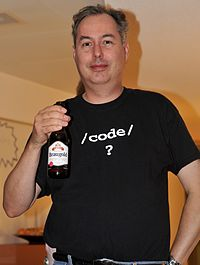
\includegraphics{Bram_Moolenaar_in_2007.jpg}
	\end{columns}	
\end{frame}

\begin{frame}{Преимущества и особенности}
	\begin{block}{Неоспоримые преимущества}
	\begin{itemize}
		\item{Работает везде}
		\item{Очень логичен}
		\item{Необыкновенно удобен}
		\item{Настраиваем и расширяем}
		\item{Хорошо работает с большими файлами. Попробуйте открыть текстовый файл размером в 1Gb}
	\end{itemize}
	\end{block}
	\begin{block}{Особенности}
	\begin{itemize}
		\item{Модален}
		\item{Больше предназначен для \alert{редактирования} текста}
		\item{Высокий порог входа}
	\end{itemize}
	\end{block}

\end{frame}

\begin{frame}{Введение}
	Знакомство с VIM

	\begin{columns}[c]

	\begin{column}{.4\textwidth}
		%\begin{block}{Способы запуска Vim}
	%\fbox{
	\begin{enumerate}
		\item
			%\begin{theorem}
				vim имя файла
			%\end{theorem}
		\item vimdiff Имя1 Имя2
	\end{enumerate}%}
	%\end{block}
	\end{column}

	\begin{column}{.6\textwidth}
	\fbox{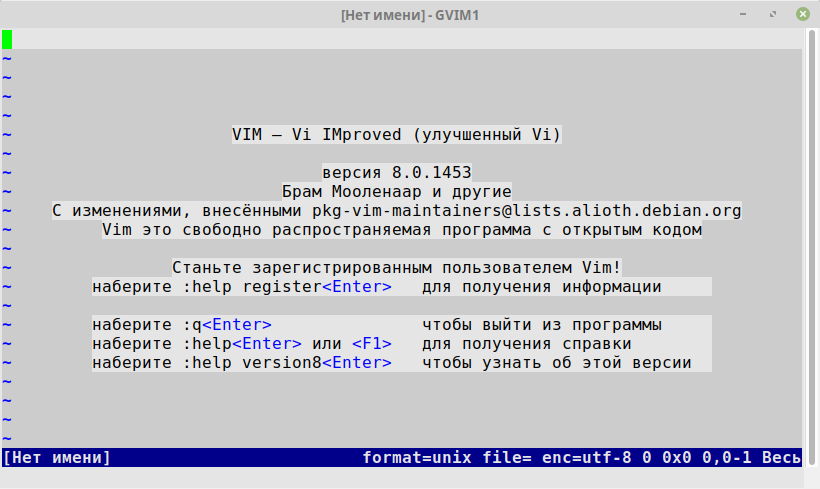
\includegraphics[width=\textwidth]{vim.png}}%
	\end{column}

	\end{columns}
\end{frame}

\begin{frame}{Режимы (modes)}	% Режимы работы редактора
\begin{columns}[c]
\column{.6\textwidth}
	\begin{itemize}
	\item<1-2>«Обычный режим» --- перемещение по файлу, стирание текста и другие редактирующие функции. Это — основной режим, только из него можно сразу перейти в другие режимы.
	\item<1-2>
	«Режим ввода» --- ввод текста. %Как только завершается ввод текста, принято сразу возвращаться в обычный режим. 
	\item<1-2>«Визуальный режим» --- режим выделения текста.
	\item<2->«Командный режим» --- Команды (операции с файлом, поиск и замена, настройка редактора…).
	\item<2->«Режим поиска» --- ввод поискового запроса.
	\end{itemize}
\column{.4\textwidth}
\tikzstyle{mode}=[rectangle,rounded corners,thick,minimum size=1cm, scale=.75, draw]
\tikzstyle{name to}=[text=red,auto] % Стиль подписи "Туда"
\tikzstyle{name out}=[text=blue,auto] % Стиль подписи "Обратно"
\tikzset{to line/.style={color=red}}% Стиль стрелки "Туда"
\tikzset{out line/.style={color=blue}}% Стиль стрелки "Обратно"
\begin{tikzpicture}[text height=1em,node distance=1.5cm and .5cm]%[thick,node distance=1.5cm and .5cm,text height=1ex ,auto]
\node<1-2>[mode](normal){Обычный};
\node<1-2>[mode,above right=of normal](input){Ввод};
\node<2>[mode,above=of normal,yshift=5pt](find){Поиск};
\node<2>[mode,right=of normal](comand){Командный};
\node<1-2>[mode,below=of normal](visual){Визуальный};

\draw<2->[to line][->](normal) to  node[name to]{:}  (comand);
%\path(normal) edge[->] (input);
\draw<1-2>[to line] [->] (normal) to  [out=90, in=270] node[yshift=5pt][name to][swap]{i,a,I,A,s,c} (input);
\draw<1-2>[out line] [->] (input) to  [out=180, in=135] node[yshift=15pt,xshift=5pt,node font=\itshape][name out]{<Esc>} (normal);
\draw<2>[to line] [->] (normal) to [out=165, in=180] node[name to][swap]{/,?} (find);
\draw<1-2>[to line] [->](normal) to node[name to]{v} node[name to][swap]{V} (visual) ;
\draw<1-2>[out line] [->](visual) to [out=180, in=195] node[name out][swap]{<Esc>} (normal) ;
\draw<2>[out line] [->](comand) to [out=225, in=315]  node[name out,yshift=5pt,node font=\small]{<Esc>} (normal) ;
\draw<2>[to line][->](visual) to [out=0, in=270] node[name to]{:} (comand);
\begin{pgfonlayer}{background}
	\node<1>[fill=gray!20,
	fit=(normal) (input) (visual)]{};
	\node<2>[fill=gray!20,
	fit=(normal) (input) (visual) (find) (comand)]{};
\end{pgfonlayer}
\end{tikzpicture}
\end{columns}
\end{frame}

\begin{frame}{Работа с несколькими файлами}
	Открытый файл в Vim называется буфером. Одновременно можно работать с несколькими буферами разными способами.\\
	Один и тот же файл можно открыть в нескольких буферах. Иногда это полезно при работе с большими файлами.
	\begin{itemize}
		\itemСразу открывается несколько файлов, но работа происходит только в одном. Переключение между буферами происходит командами:next,prev
		\itemОкно экрана разделяется на несколько частей. В каждом окне можно открыть свой буфер.
		\itemКаждый буфер открывается в своей вкладке.
	\end{itemize}
	%\includegraphics<1>[width=\textwidth]{many_files.png}
	%\includegraphics<2>[width=\textwidth]{tab_files.png}
\end{frame}

\begin{frame}{Текстовые объекты}\label{objects}
	Редактор Vim умеет работать с разными сущностями. \\
	Это:
	\begin{itemize}
		\itemСимвол;
		\itemСлово --- несколько символов, отделенных друг от друга пробельными символами;
		\itemСтрока --- несколько символов, отделенных друг от друга символом конца строки;
		\itemПредложение --- несколько слов отделенных друг от друга знаками препинания, которыми может заканчиваться предложение;
		\itemПараграф --- несколько предложений отделенных друг от друга пустой строкой или командой окончания абзаца;
		\itemБлок текста --- текст заключенный в парные скобки;
		\itemФайл.
	\end{itemize}
\end{frame}

\begin{frame}[fragile]{Перемещение по тексту (обычный режим)}
	Рассмотренные на предыдущем слайде \hyperlink{objects}{объекты} могут быть единицами перемещения по тексту.

	Некоторые примеры перемещения по тексту в редакторе: \\
\begin{itemize}
	\item<2->К началу следующего слова;
	\item<3->К концу текущего слова;
	\item<4->К началу предложения;
	\item<5->К началу следующего предложения.
\end{itemize}

\begin{tikzpicture}%[thick,node distance=2cm and .5cm,text height=1.5ex, auto]
		[thick,%decoration=snake,
		auto,
		source letter/.style = {rectangle,fill=blue!20},
		target letter/.style = {rectangle,fill=green!30},
		command/.style = {rectangle,fill=red!40,draw=blue}]

	\matrix[draw=red,matrix of nodes,column sep={.7em,between origins}]
	{
		P&r&o&b&a&&\node<1>{t};\node<2->(begin text){t};&e&x&t&.&&И&с&с&л&е&д&у&е&м&&п&е&р&е&м&е&щ&е&н&и&я&.&&&&&\\
		\node<-3>{Н};\node<4->[target letter](this sequence){Н};&а&&\node<1>{с};\node<2->[source letter](source position){с};&л&е&д&у&ю&щ&е&\node<-2>{й};\node<3->[target letter](end word){й};&&\node<1>{с};\node<2->[target letter](begin too){с};&т&р&о&к&е&.&&\node<-4>{С};\node<5->[target letter](next sequence){С};&л&е&д&у&ю&щ&е&е&&&&&&&&&& \\
		п&р&е&д&л&о&ж&е&н&и&е& &н&а& &н&о&в&о&й& &с&т&р&о&к&е&.&&Е&щ&ё&&с&л&о&в&а&.&\\
	}; 
	%\draw[->](begin text) to (begin too);
	\path<2->[->](source position) edge [bend left=15] node[command,above, yshift=2pt] {w} (begin too);
	\path<3->[->](source position) edge [bend right] node[command,below, yshift=-2pt] {e} (end word);
	\path<4->[->](source position) edge [out=110, in=45] node[command,above, yshift=2pt] {(} (this sequence);
	\path<5->[->](source position) edge [bend left=45] node[command,above, yshift=2pt] {)} (next sequence);

\end{tikzpicture}\\

\end{frame}

\begin{frame}[fragile]{Работа в визуальном режиме}
	\begin{itemize}
	\item<2-> Выделение слова (\verb:viw:);
	\item<3-> Выделение большого слова (\verb:vaw:);
	\item<4-> Выделение строки (\verb:V:);
	\item<5-> Выделение блока в круглых скобках (\verb:vib:);
	\item<6-> Выделение блока в фигурных скобках (\verb:viB:);
	\end{itemize}
	%Код программы на Си:

\begin{tikzpicture}[auto,font=\small,
			inner sep = 1pt,
			green back/.style = {rectangle, fill=green!20},
			gray back/.style = {rectangle, fill=gray!20}]
	\matrix[draw=red,matrix of nodes,column sep={.7em,between origins}, row sep={1em,between origins}]
	{
%	a&a&a&\\
%#define	FLAG_END_KEYBOARD_COD	0	// Флаг выставляется при срабатывании таймера
\#&d&e&f&i&n&e&	&F&L&A&G&\_&A&L&T&\_&K&E&Y& &1&&&/&/& &Ф&л&а&г& &к&л&а&в&и&ш&и&\\
v&o&l&a&t&i&l&e& &u&i&n&t&8&\_&t& &f&l&a&g&s& &=& &0&;&\\
%volatile static uint8_t receive_cod[10]={0,0,0,0,0,0,0,0,0,0}; // Массив для хранения полученного от клавиатуры кода
%volatile static uint8_t *p_byte;	// Указатель показывает на элемент массива, с которым производится действие
%volatile static uint8_t stack_keys[SIZE_STACK_KEY]={0,0,0,0,0,0,0,0,0,0}; // Массив для хранения стека нажатых клавиш
%volatile static uint8_t *p_key;		// Указатель на элемент стека клавиш
\node(1-0){v};&\node(1-1){o};&\node(1-2){i};&\node(1-3){d};&\node(1-4){ };&\node(1-5){s};&\node(1-6){t};&\node(1-7){a};&\node(1-8){r};&\node(1-9){t};&\_&\node(1-10){t};&\node(1-11){i};&\node(1-12){m};&\node(1-13){e};&\node(1-14){r};&\node(1-15){0};&&&\\
\{&&&&&&&&&&&&&&&&&&&&&&&&\\
&&&\node(0-0){T};&\node(0-1){C};&\node(0-3){N};&\node(0-4){T};&\node(0-5){0};&\node(0-6){ };&&\node(0-7){=};&\node(0-8){ };&&\node(0-9){S};&\node(0-10){T};&\node(0-12){A};&\node(0-13){R};&\node(0-14){T};&\node(0-15){\_};&\node(0-16){T};&\node(0-17){C};&\node(0-18){N};&\node(0-19){T};&\node(0-20){0};&\node(0-21){;};&\\
&&&T&I&F&R& &&\textbar&=& &&(&1& &<&<& &T&O&V&0&)&;&\\
&&&T&I&M&S&K& &\textbar&=& &&(&1& &<&<& &T&O&I&E&0&)&;&\\
&&&\node(4-0){T};&\node(4-1){C};&\node(4-2){C};&\node(4-3){R};&\node(4-4){0};&\node(4-5){ };&\node(4-6){\&};&\node(4-7){=};& &\node(4-8){\textasciitilde};&\node(4-9){(};&\node(4-10){1};&\node(4-11){ };&\node(4-12){<};&\node(4-13){<};&\node(4-14){ };&\node(4-15){C};&\node<1>[green back](4-16)(place cursor){S};\node<2->(4-17){S};&\node(4-18){0};&\node(4-19){1};&\node(4-20){)};&\node(4-21){;};&\\
&&&\node(3-0){T};&\node(3-1){C};&\node(3-2){C};&\node(3-3){R};&\node(3-4){0};&\node(3-5){ };&\node(3-6){\textbar};&\node(3-7){=};&\node(3-8){ };&&(&\node(3-9){1};&\node(3-10){ };&\node(3-11){<};&\node(3-12){<};&\node(3-13){ };&\node(3-14){C};&\node(3-15){S};&\node(3-16){0};&\node(3-17){2};&\node(3-11){)};&\node(3-18){\textbar};&(&\node(3-19){1};&\node(3-20){ };&\node(3-21){<};&\node(3-22){<};&\node(3-23){ };&\node(3-24){C};&\node(3-25){S};&\node(3-26){0};&\node(3-27){0};&\node(3-28){)};&\node(3-29){;};&\\
\}&&&&&&&&&&&&&&&&&&&&&&&&&\\
};
\begin{pgfonlayer}{background}
	\node<2->[fill=gray!40,
	fit=(4-15) (4-17) (4-18) (4-19)]{};
	\node<3-4,6>[fill=gray!40,
	fit=(4-20) (4-21)]{};
	\node<4->[fill=gray!40,fit=(4-10) (4-11) (4-12) (4-13) (4-14)]{};
	\node<6>[fill=gray!40,fit= (0-0) (0-1) (0-3) (0-4) (0-5) (0-6) (0-7) (0-8) (0-9) (0-10) (0-12) (0-13) (0-14) (0-15) (0-16) (0-17) (0-18) (0-19) (0-20) (0-21) % 
	(3-0) (3-1) (3-2) (3-3) (3-4) (3-5) (3-6) (3-7) (3-8) (3-9) (3-10) (3-11) (3-12) (3-13) (3-14) (3-15) (3-16) (3-17) (3-18) (3-19) (3-20) (3-21) (3-22) (3-23) (3-24) (3-25) (3-26) (3-27) (3-28) (3-29)]{};
	\node<4,6>[fill=gray!40,fit=(4-0) (4-1) (4-2) (4-3) (4-4) (4-5) (4-6) (4-7) (4-8) (4-9)]{};
\end{pgfonlayer}

\end{tikzpicture}

\end{frame}

\begin{frame}{Командный режим редактора}
Режим работы в текстовом редакторе Ex\\
Чаще всего используемые команды:
\begin{itemize}
\item :s;
\item
\end{itemize}
\end{frame}

\begin{frame}{Философия редактора Vim}
\end{frame}

\begin{frame}{Обобщенный формат команды}
\end{frame}

\begin{frame}{Взаимодействие с окружающей средой}

\begin{iteemize}
\item Вставка в текст результатов выполнения команды ОС;
\item Обработка редактируемого текста внешней командой;
\item Интеграция оболочки;
\item Использование внешних инструментов проверки текста;
\item Компиляция и сборка программ;
\item Обработка ошибок.
\end{itemize
\end{frame}

\begin{frame}{Семейство приложений а ля Vimo}
\begin{enumerate}
\item Интернет-просмотрщик --- vimperator;
\item Просмотршик pdf, djvu файлов --- zathura;
\item Файловый менеджер --- vifm;
\item Редактор командной строки Linux --- set -o vi.
\end{enumerate}
\end{frame}

\begin{frame}{Литература}
Есть две рускоязычные книги про Vim:
\begin{itemize}
\item
	\parbox[c]{.6\textwidth}{
Автор:Дрю Нейл\\
Практическое использование Vim\\
ISBN: 978-5-94074-972-1
}
\begin{minipage}{.3\linewidth}
		\includegraphics[height=.2\textheight]{Practic_Vim.jpg}
\end{minipage}
\item
	\begin{minipage}{.6\textwidth}
Авторы:Арнольд Роббинс, Линда Лэмб, Элберт Ханна\\
Изучаем редакторы vi и Vim. 7-е издание\\
ISBN: 978-5-93286-200-1
\end{minipage}
\begin{minipage}{.3\linewidth}
		\includegraphics[height=.2\textheight]{Learn_Vim.jpg}
\end{minipage}
\end{itemize}
\end{frame}

\end{document}
